\subsection{Vision Detection Principles}
% vision hardware set up + software implementation
In order to achieve the vision detection task we had broken down the task into 4 sub tasks as follows:
\begin{enumerate}
	\item Identify the Cards on the table.
	\item Coordinates and pose of the cards.
	\item Match the local coordinates to the world coordinates.
	\item Identify the features of the cards.
\end{enumerate}


1.	Identify the cards on the table.
\begin{itemize}
	\item In the initial sweep after hiding the robot arm the camera will capture an image of the table. Histogram equalisation has been used to equalise the intensity over the image to make the image processing task easier. 
	\item The back of the card gives pixel values that are very close to black as represented in a a grayscale image. Using this data a logical image has been created by using a threshold of pixel values less than 0.09. After removing continuous pixel groupings with areas less than 1000, \emph{bwareopen} a structured element has been used to morphologically close the founded blobs.
	\item •	The same logic has been used to find face up cards as well but with a threshold of 0.91 to choose cards that are white in colour (and therefore are face up).
\end{itemize}

\begin{figure}[position = here]
	\begin{centering}
		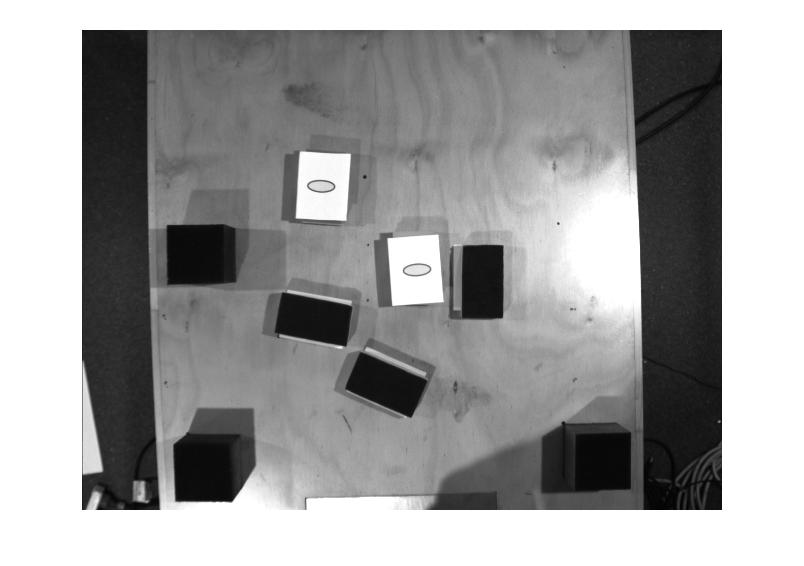
\includegraphics[scale=0.3]{./sachiths_images/image3.png}\\
		\caption[]{\textit{Initial captured image}}
	\end{centering}
\end{figure}

\begin{figure}[position = here]
	\begin{centering}
		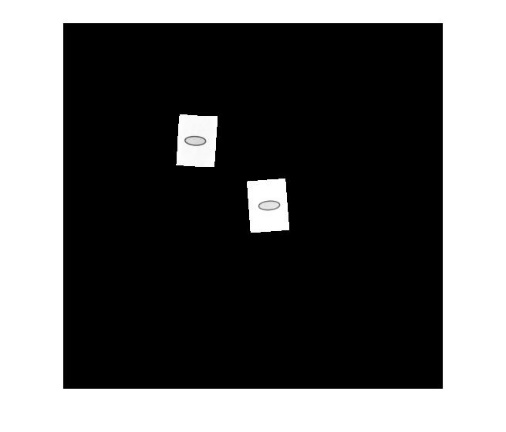
\includegraphics[scale=0.9]{./sachiths_images/image32.png}\\
		\caption[]{\textit{Isolated Cards}}
	\end{centering}
\end{figure}

2.	Coordinates and Pose of the cards
\begin{itemize}
	\item A logical image was created using the aforementioned methodand this image was then used to find the local centroids and the orientations of the cards. The function \emph{regionprops} has been used to find the centroids and orientation. After finding both, centroids and orientations of the fiducials have been removed from our collection in order to present the collection of cards back to the Card data structure. In orientations a redundancy has been added to make sure that the robot arm will always work in the safety limits by checking the value of the angle and deciding the shortest path to the desired gripper angle (in order to stop the arm from over-revolving around joint 4 and damaging the pneumatic lines that control the end effector action).
	
\end{itemize}

3.	Match the local coordinates to the world coordinates
\begin{itemize}
	\item Three fiducials have been used to get the relative position of the cards by using two fiducials at a time to create two theoretical axes (the lines formed between them) and then using a perpendicular distance calculation to find the real world position of each card as seen in Figure\ref{trilatAlternate}. This is a simplification of the trilateration issue that we have encountered in the past with this Epson arm setup.
	
\end{itemize}
\begin{figure}[position = here]
	\begin{centering}
		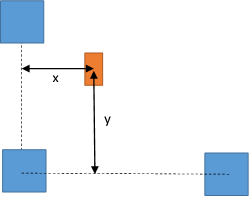
\includegraphics[scale=0.8]{./sachiths_images/image4.png}\\
		\caption[]{\textit{Method used to match with world coordinates\label{trilatAlternate}}}
	\end{centering}
\end{figure}

4.	Identify the features of the cards
\begin{itemize}
	\item The main target was to identify the card itself before trying to extract features which used the same method as above to identify the card using pixel values as thresholds. We could then use the discorvered logical image as a mask to isolate only the card face that was relevant to us. This is one of the major advantages of using the peek-unpeek method as it is easier to control mechanically than to flip in place and the vision detection is simplified by being told exactly where to apply the masks.

\end{itemize}
\begin{figure}[position = here]
	\begin{centering}
		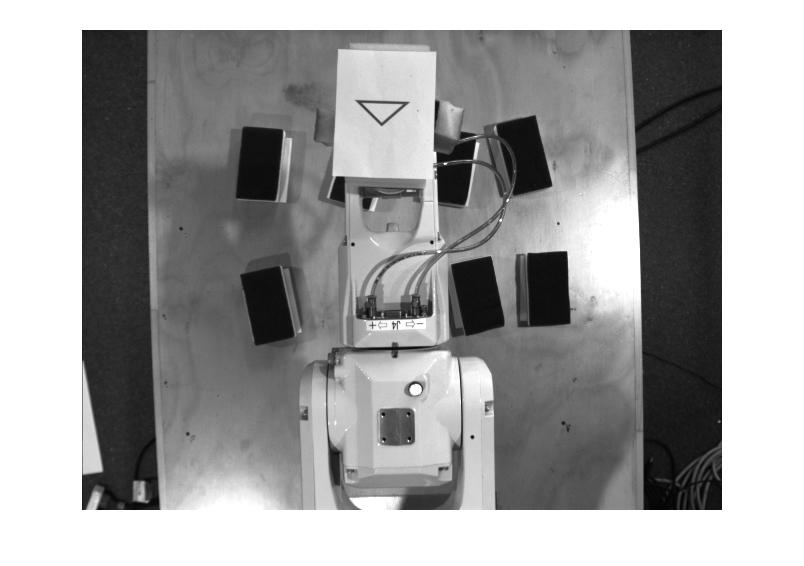
\includegraphics[scale=0.3]{./sachiths_images/image5.png}\\
		\caption[]{\textit{Initial image of the faceup card\label{imFup1}}}
	\end{centering}
\end{figure}
\begin{figure}[position = here]
	\begin{centering}
		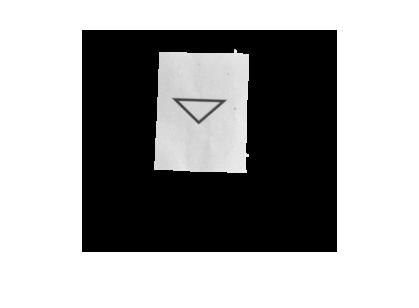
\includegraphics[scale=0.5]{./sachiths_images/image6.png}\\
		\caption[]{\textit{Isolated Card\label{isol1}}}
	\end{centering}
\end{figure}

\begin{itemize}
	\item From this image a bounding box was used to crop out the card to process it for the features of shape, shape count and filler.
\end{itemize}

\begin{itemize}
	\item Edge detection has been used to find the shape. After detecting the edges of the shape unnecessary edges has been removed using clearing edges connected to border and removing connected regions less than a threshold pixel area.
	
\end{itemize}
\begin{figure}[position = here]
	\begin{centering}
		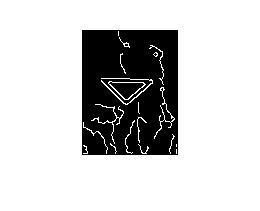
\includegraphics[scale=0.8]{./sachiths_images/image10.jpg}\\
		\caption[]{\textit{Identified Edges}}
	\end{centering}
\end{figure}
\begin{figure}[position = here]
	\begin{centering}
		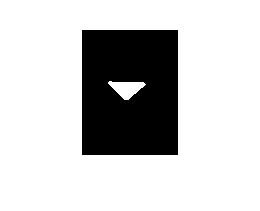
\includegraphics[scale=0.8]{./sachiths_images/image11.jpg}\\
		\caption[]{\textit{Identified Shape}}
	\end{centering}
\end{figure}
\begin{itemize}
	\item Perimeter of the discovered blob was used to identify the shape as triangle, rectangle and ellipse had different perimeter values. Number of connected components in this stage has been used to identify the shape count. If the shape count is greater than 1, the mean perimeter will be checked for identify the shape. The final logical image with the shape has been used with the original image to identify the filler status. Mean intensity of the blob area of the logical image in original image will have a value greater than 0.72 if the shape is not shaded as pixel value for white is 1. For block status the mean intensity will be lowest and for shaded status the intensity value will be between 0.72 and 0.5.
	
	
\end{itemize}
	